\documentclass[tikz,border=8pt]{standalone}
\usetikzlibrary{shapes.geometric,arrows.meta,positioning}
\begin{document}
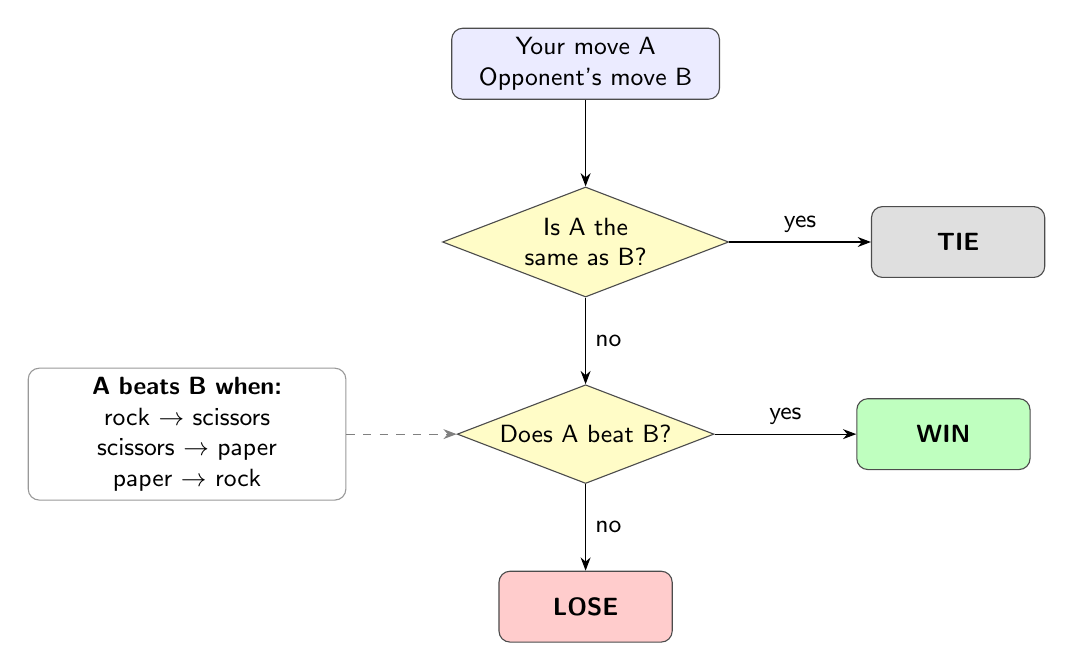
\begin{tikzpicture}[
  font=\sffamily\small, >=Stealth,
  box/.style={rectangle,rounded corners,draw=black!70,fill=blue!8,align=center,minimum height=9mm,minimum width=34mm},
  ask/.style={diamond,aspect=2.6,draw=black!70,fill=yellow!22,align=center,inner sep=2pt},
  res/.style={rectangle,rounded corners,draw=black!70,align=center,minimum height=9mm,minimum width=22mm,font=\sffamily\bfseries\small},
  node distance=11mm and 18mm]
\node[box] (start) {Your move A\\Opponent's move B};
\node[ask,below=of start] (same) {Is A the\\same as B?};
\node[res,fill=gray!25,right=of same] (tie) {TIE};
\node[ask,below=of same] (beat) {Does A beat B?};
\node[res,fill=green!25,right=of beat] (win) {WIN};
\node[res,fill=red!20,below=of beat] (lose) {LOSE};
\node[box,fill=white,draw=black!40,left=14mm of beat,text width=38mm] (rule)
  {\textbf{A beats B when:}\\rock $\to$ scissors\\scissors $\to$ paper\\paper $\to$ rock};
\draw[->] (start)--(same);
\draw[->] (same)--node[above]{yes}(tie);
\draw[->] (same)--node[right]{no}(beat);
\draw[->] (beat)--node[above]{yes}(win);
\draw[->] (beat)--node[right]{no}(lose);
\draw[dashed,->,black!50] (rule)--(beat);
\end{tikzpicture}
\end{document}
